\documentclass[12pt]{article}
\usepackage[T1]{fontenc}
\usepackage{geometry}
\geometry{verbose, a4paper, tmargin=1.3in, bmargin=0.85in, lmargin=1.4in, rmargin=0.85in}
\usepackage{lscape}
\usepackage{fancyvrb}
\usepackage{lineno,hyperref}
\usepackage{graphics}
\usepackage{graphicx}
\usepackage{epsfig}
\usepackage{amsmath}  
\usepackage{amsfonts}
\usepackage{amsthm} 
\usepackage{amssymb}
\usepackage{placeins}
\usepackage{multirow}
\usepackage[export]{adjustbox}[2011/08/13]
\usepackage{tabularx}
\usepackage{fancyvrb}
\usepackage{caption}
\usepackage{epsf}
\usepackage{epstopdf}
\usepackage{subfigure} 
\usepackage{colortbl}
\usepackage{longtable}
\usepackage{enumerate}
\usepackage{tabularx, booktabs}
\usepackage{url}
\usepackage{graphicx}
\usepackage{setspace}
\usepackage{float}
\usepackage{enumitem}
\usepackage{listings}
\usepackage{xcolor} 

\usepackage{longtable}
\usepackage{color}
\definecolor{highlight}{RGB}{255, 255, 204}

\documentclass{article}
\usepackage{tikz}
\usetikzlibrary{automata, positioning}
\usepackage{multirow}
\usepackage[flushleft]{threeparttable}
\usepackage{multicol}
\usepackage{multirow}
\usepackage{array, makecell}
\usepackage{hhline}
\usepackage{longtable}
\usepackage{tabularray}
\usepackage[table,xcdraw]{xcolor}
\usepackage{caption}

% Page Border
\usepackage{tikz}
\usetikzlibrary{calc}
\newcommand\HRule{\rule{\textwidth}{1pt}}
\usepackage{tabularx}
\usepackage{longtable}
\newcolumntype{P}[1]{>{\centering\arraybackslash}m{#1}}
\usepackage{tcolorbox}
% To set Figure Caption and Text Gap
\setlength\belowcaptionskip{2ex}
% \linespread{1.1}


\newlength{\defbaselineskip}
\setlength{\defbaselineskip}{\baselineskip}
\newcommand{\setlinespacing}[1]{\setlength{\baselineskip}{#1 \defbaselineskip}}

\usepackage{makecell}
\newcounter{qcounter}
\usepackage{enumitem}
\usepackage{hyperref}
\usepackage{multirow}
\usepackage{xcolor}



% Table caption below the table
\begin{document}
\begin{titlepage}
\begin{center}
{\fontsize{22}{26.4}\textbf{A Report on\ Compiler Design Lab (CS304) Mini Project}}\\
\textbf{}\\
{\textbf{M Vineet Nayak}} (Roll No: 231CS132)\\
\vspace{0.5cm}
{\textbf{Prahas GR}} (Roll No: 231CS142)\\
\vspace{0.5cm}
{\textbf{Nischal Basavaraju}} (Roll No: 231CS139)\\
\vspace{0.3cm}
\begin{figure}[h]
{\centering {\includegraphics[height=4.5cm]{nitk_logo.png}}\par}
\end{figure}
\setstretch{2}
{\textbf{DEPARTMENT OF COMPUTER SCIENCE AND ENGINEERING}\par}
\vspace{-12pt}
{\textbf{NATIONAL INSTITUTE OF TECHNOLOGY KARNATAKA}\par}
\vspace{-12pt}
{\textbf{SURATHKAL, MANGALURU-575025}\par}
\vspace{-12pt}
{\textbf{13-August-2025}\par}
\end{center}
\pagebreak
\end{titlepage}



\tableofcontents
\newpage










\section{Introduction} 
\subsection{Lexical Analysis}
Lexical analysis is the first stage of the compiler where the source code is scanned and broken down into smaller meaningful units. This process converts a sequence of characters into a sequence of tokens, which can then be used by the parser in later stages of compilation. The lexical analyzer also removes whitespace and comments, and reports errors for invalid tokens.

\subsection{Tokens \& Lexemes}
A token is a classified unit of code that represents a category of symbols defined in the programming language. Common token types include keywords, identifiers, constants, operators, and punctuation symbols. Each token is recognized by a specific pattern, such as a regular expression, defined in the lexical analyzer.

A lexeme is the actual sequence of characters in the source code that matches the pattern of a token. For example, in the line int x = 5;, the lexemes are int, x, =, and 5, which correspond to the tokens keyword, identifier, operator, and constant, respectively.

\section{Implementation}
This part of the project has been implemented using Flex, where regular expressions are written to define the patterns of tokens. The Flex code is then compiled into equivalent C code for execution. The program takes a C source file as input and, for each token encountered, prints its details. At the end of execution, it also generates and displays a symbol table and a constant table.

\subsection{Scanner Code}
The entire code for the project can be found at www.github.com/vin06eet/Compiler\_Design 


\subsection{List of Recognized Tokens}
The following categories of tokens are recognized by the scanner:
\begin{itemize}
    \item \textbf{Identifiers: } variable names, function names
    \item \textbf{Keywords: } if, else, while, for, int, char, return, etc.
    \item \textbf{Constants: } numeric, string, character literals
    \item \textbf{Preprocessor directives: } \#include, \#define
    \item \textbf{Operators: } +, -, *, /, =, ==
    \item \textbf{Punctuation symbols: } parentheses, braces, commas, semicolons
\end{itemize}

\subsection{DFA Diagram}

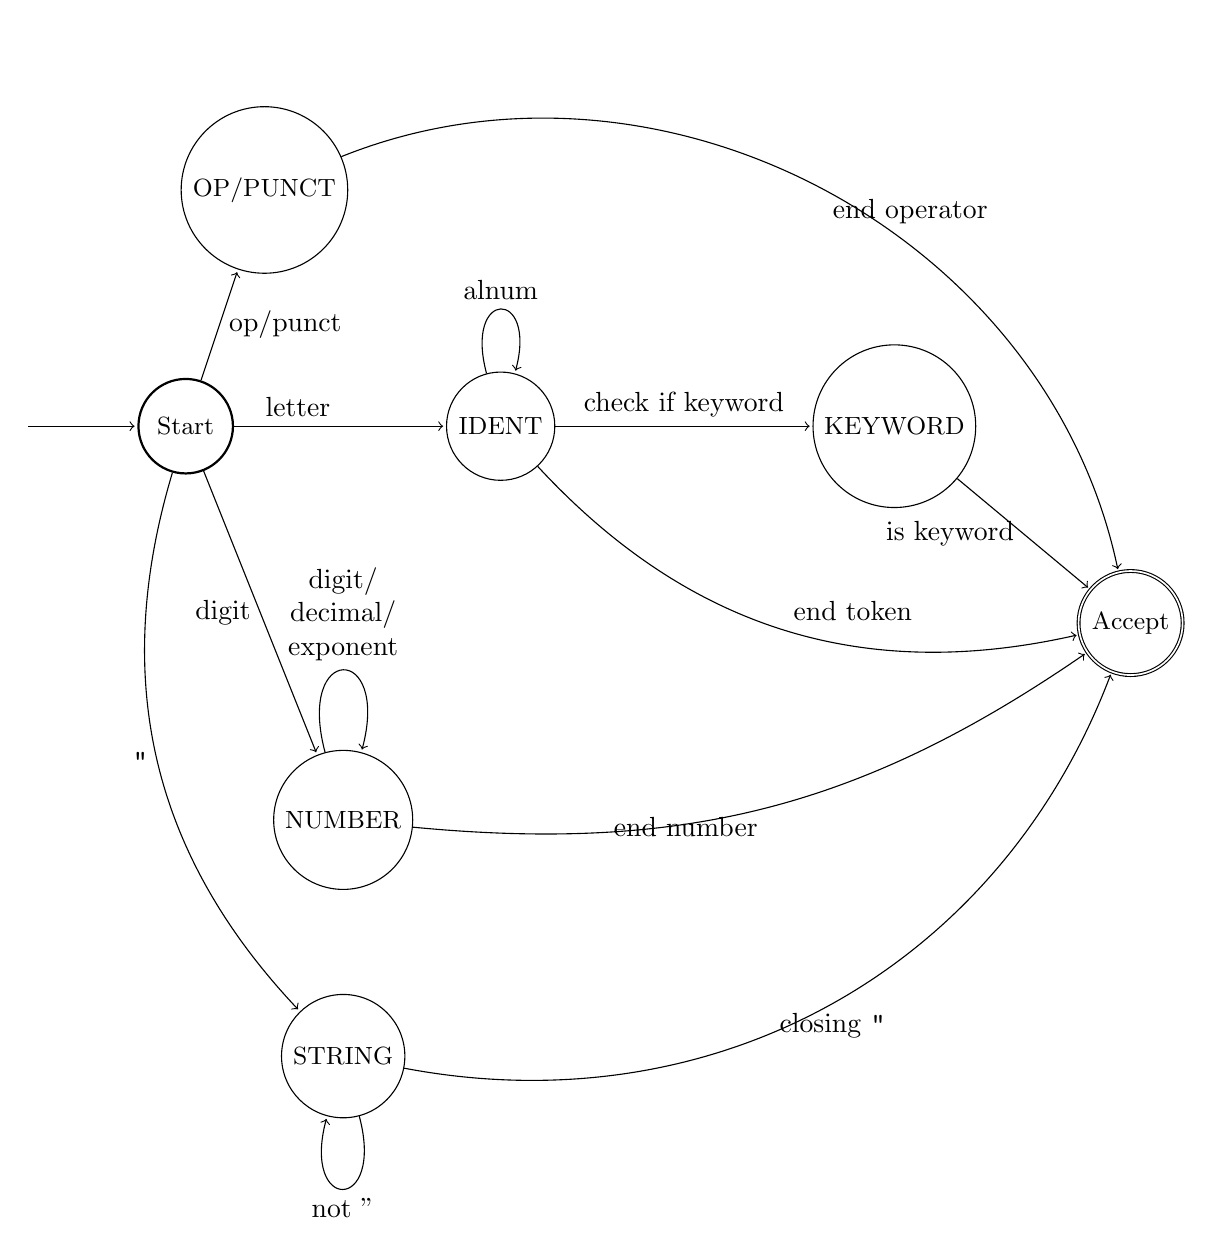
\begin{tikzpicture}[
    shorten >=1pt, 
    node distance=4cm, 
    on grid, 
    auto,
    state/.style={circle, draw, minimum size=1.2cm, font=\small},
    initial/.style={state, thick},
    accepting/.style={state, double}
]
  % States positioned for better layout
  \node[state, initial] (start) {Start};
  \node[state] (ident)  [right=4cm of start] {IDENT};
  \node[state] (kw)     [right=5cm of ident] {KEYWORD};
  \node[state, accepting] (acc) [below right=2.5cm and 3cm of kw] {Accept};
  \node[state] (op)     [above right=3cm and 1cm of start] {OP/PUNCT};
  \node[state] (num)    [below right=5cm and 2cm of start] {NUMBER};
  \node[state] (string) [below=3cm of num] {STRING};
  \draw[->] (-2,0) -- (start);
  
  % Transitions from Start

  \path[->]
    (start) edge node[above left] {letter} (ident)
            edge node[left] {digit} (num)
            edge[bend right=30] node[left] {\texttt{"}} (string)
            edge node[right] {op/punct} (op);
  
  % IDENT transitions
  \path[->]
    (ident) edge[loop above] node {alnum} (ident)
            edge node[above] {check if keyword} (kw)
            edge[bend right=30] node[above right] {end token} (acc);
  
  % KEYWORD to Accept
  \path[->]
    (kw) edge node[left] {is keyword} (acc);
  
  % NUMBER transitions
  \path[->]
    (num) edge[loop above] node[align=center] {digit/\\decimal/\\exponent} (num)
          edge[bend right=20] node[below left] {end number} (acc);
  \path[->]
    (string) edge[loop below] node[align=center]
    {not "} (string);
  % STRING to Accept
  \path[->]
    (string) edge[bend right=40] node[below] {closing \texttt{"}} (acc);
  
  % OP/PUNCT to Accept
  \path[->]
    (op) edge[bend left=50] node[below right] {end operator} (acc);
\end{tikzpicture}

\subsection{Assumptions}
The scanner assumes a C89/C90-like subset of the C language and does not fully implement C99/C11 features. It supports both block comments (/* ... */) and line comments (// ...), with additional support for nested comments (non-standard in C). The preprocessor is only partially supported: \#define constants are recognized, while other directives are tokenized without further semantic processing. Identifiers in declarations are treated as types only on their first occurrence, and multi-word types (e.g., \texttt{unsigned int}) are concatenated. Function parameters are captured as raw strings, with multiple parameters separated by semicolons. Array dimensions are appended only when specified immediately after an identifier (e.g., \texttt{arr[10]}). Numeric constants with suffixes (u, l, f, etc.) are recognized, though suffixes do not affect type classification beyond token recognition. The scanner does not handle trigraphs or digraphs. Errors such as unterminated strings, characters, comments, or invalid tokens are reported, but scanning continues to allow recovery. Whitespace inside array dimension brackets (e.g., \texttt{[ 10 ]}) is permitted.

\section{Results}
Several files were given as input to the scanner, and the outputs of some of the C codes are given below.
\subsection{Test Case 1: Simple Program}
Input:
\begin{verbatim}
int main() {
    int a = 100;
    float b = 2.532;
    char c = 'c';
    return a + b;
}
\end{verbatim}
Output:
\begin{lstlisting}[basicstyle=\ttfamily\small]
[line 1] TYPE         : int
[line 1] IDENT        : main
[line 1] PUNCT        : (
[line 1] PUNCT        : )
[line 1] PUNCT        : {
[line 2] TYPE         : int
[line 2] IDENT        : a
[line 2] OP           : =
[line 2] NUMBER       : 100
[line 2] PUNCT        : ;
[line 3] TYPE         : float
[line 3] IDENT        : b
[line 3] OP           : =
[line 3] NUMBER       : 2.532
[line 3] PUNCT        : ;
[line 4] TYPE         : char
[line 4] IDENT        : c
[line 4] OP           : =
[line 4] CHAR         : 'c'
[line 4] PUNCT        : ;
[line 5] KEYWORD      : return
[line 5] IDENT        : a
[line 5] OP           : +
[line 5] IDENT        : b
[line 5] PUNCT        : ;
[line 6] PUNCT        : }
\end{lstlisting}
\vspace{3em}
\bigskip
\textbf{Symbol Table:}
\begin{center}
\begin{tabular}{|l|l|l|c|l|l|}
\hline
Name & Type & Dimension & Frequency & Return Type & Parameters \\
\hline
a    & int   & -  & 2 & - & - \\
b    & float & -  & 2 & - & - \\
c    & char  & -  & 2 & - & - \\
main & int   & - & 1 & function &  \\
\hline
\end{tabular}
\end{center}

\bigskip
\textbf{Constant Table:}
\begin{center}
\begin{tabular}{|l|l|l|c|}
\hline
Variable Name & Line No. & Value  & Type \\
\hline
not\_allowed & 3  & 5   & int \\
- & 4 & 0 & int \\
\hline
\end{tabular}
\end{center}

\subsection{Test Case 2: With Errors}
Input:
\begin{verbatim}
int main() {
    string s = "Howdy; // wrong syntax for string declaration
    @not_allowed = 5;     // invalid identifier, cannot start with @
    return 0;
}
\end{verbatim}

Output:
\begin{lstlisting}[basicstyle=\ttfamily\small]
[line 1] TYPE         : int
[line 1] IDENT        : main
[line 1] PUNCT        : (
[line 1] PUNCT        : {
[line 2] IDENT        : string
[line 2] IDENT        : s
[line 2] OP           : =
[line 2] ERROR: Unterminated string literal
[line 3] ERROR: Invalid token '@'
[line 3] IDENT        : not_allowed
[line 3] OP           : =
[line 3] NUMBER       : 5
[line 3] PUNCT        : ;
[line 4] KEYWORD      : return
[line 4] NUMBER       : 0
[line 4] PUNCT        : ;

[line 5] PUNCT        : }
\end{lstlisting}
%% Continue your report section

\bigskip
\textbf{Symbol Table:}
\begin{center}
\begin{tabular}{|l|l|l|c|l|l|}
\hline
Name & Type & Dimension & Frequency & Return Type & Parameters \\
\hline
string    & -   & -  & 1 & - & - \\
s    & - & -  & 1 & - & - \\
not\_allowed    & -  & -  & 1 & - & - \\
main & int   & - & 1 & function &  \\
\hline
\end{tabular}
\end{center}

\bigskip
\textbf{Constant Table (excerpt):}
\begin{center}
\begin{tabular}{|l|l|l|c|}
\hline
Variable Name & Line No. & Value  & Type \\
\hline
a & 2  & 100   & int \\
b & 3 & 2.532 & float \\
c & 4 & 'c'  & char \\
\hline
\end{tabular}
\end{center}
\vspace{1em}
\textbf{Explanation for unusual behaviour: }
    Since the scanner is designed to continue scanning even after detecting an error, some invalid tokens may still be recognized and added to the symbol or constant table. As a result, these tables may contain incorrect entries. However, this limitation can be addressed in later phases of compilation by discarding or ignoring the affected symbol and constant tables whenever an error is invoked.

\subsection{Test Case 3: With multiline comments, preprocessors and array usage}
Input:
\begin{verbatim}
#include <stdio.h>
#include <stdlib.h>
#include <stdbool.h>

int globalVar = 10;

int main(){
int arr[10] = {1, 2, 3, 4, 5, 6, 7, 8, 9, 10};
int b = 1000;
/*
This is to
show how
multiline comments are
handled
*/
return b*b*b;
}
\end{verbatim}

Output:
\begin{lstlisting}[basicstyle=\ttfamily\small]
[line 1] PREPROC      : #include <stdio.h>
[line 2] PREPROC      : #include <stdlib.h>
[line 3] PREPROC      : #include <stdbool.h>
[line 5] TYPE         : int
[line 5] IDENT        : globalVar
[line 5] OP           : =
[line 5] NUMBER       : 10
[line 5] PUNCT        : ;
[line 7] TYPE         : int
[line 7] IDENT        : main
[line 7] PUNCT        : (
[line 7] PUNCT        : {
[line 8] TYPE         : int
[line 8] IDENT        : arr
[line 8] PUNCT        : [10]
[line 8] OP           : =
[line 8] PUNCT        : {
[line 8] NUMBER       : 1
[line 8] PUNCT        : ,
[line 8] NUMBER       : 2
[line 8] PUNCT        : ,
[line 8] NUMBER       : 3
[line 8] PUNCT        : ,
[line 8] NUMBER       : 4
[line 8] PUNCT        : ,
[line 8] NUMBER       : 5
[line 8] PUNCT        : ,
[line 8] NUMBER       : 6
[line 8] PUNCT        : ,
[line 8] NUMBER       : 7
[line 8] PUNCT        : ,
[line 8] NUMBER       : 8
[line 8] PUNCT        : ,
[line 8] NUMBER       : 9
[line 8] PUNCT        : ,
[line 8] NUMBER       : 10
[line 8] PUNCT        : }
[line 8] PUNCT        : ;
[line 9] TYPE         : int
[line 9] IDENT        : b
[line 9] OP           : =
[line 9] NUMBER       : 1000
[line 9] PUNCT        : ;
[line 16] KEYWORD      : return
[line 16] IDENT        : b
[line 16] OP           : *
[line 16] IDENT        : b
[line 16] OP           : *
[line 16] IDENT        : b
[line 16] PUNCT        : ;
[line 17] PUNCT        : }

\end{lstlisting}
%% Continue your report section

\bigskip
\textbf{Symbol Table:}
\begin{center}
\begin{tabular}{|l|l|l|c|l|l|}
\hline
Name & Type & Dimension & Frequency & Return Type & Parameters \\
\hline
b    & int   & -  & 4 & - & - \\
globalVar    & int   & -  & 1 & - & - \\
arr    & int   & [10]  & 1 & - & - \\
main    & int   & -  & 1 & int &  \\
\hline
\end{tabular}
\end{center}

\bigskip
\vspace{1em}
\textbf{Constant Table (excerpt):}
\begin{center}
\begin{tabular}{|l|l|l|c|}
\hline
Variable Name & Line No. & Value  & Type \\
\hline
globalVar & 5  & 10   & int \\
- & 8 & 1 & int \\
- & 8 & 2 & int \\
- & 8 & 3 & int \\
- & 8 & 4 & int \\
- & 8 & 5 & int \\
- & 8 & 6 & int \\
- & 8 & 7 & int \\
- & 8 & 8 & int \\
- & 8 & 0 & int \\
b & 9 & 1000  & int \\
\hline
\end{tabular}
\end{center}
\vspace{1em}


% 
\end{document}
